\documentclass[12pt, letterpaper]{article}
\usepackage{graphicx} % Required for inserting images
%\usepackage[T1]{fontenc}

\usepackage{amsfonts}
\usepackage{tabularx}
\usepackage{multirow}
\usepackage{booktabs}
\usepackage{float}
\usepackage{caption}
%\usepackage{natbib}

\usepackage{polski}

\title{Programy użytkowe \\ Lista 6}

\date{}

\begin{document}
\maketitle

Rozwiązania zadań wpisz do notatki w \LaTeX{u} w następujący sposób: komenda wymagana  przez treść polecenia (wskazówka: \verb| \verb, \begin{verbatim} |), a pod nią wynikowy wykres, np.\\\\
\begin{minipage}{.9\linewidth}
   Zadanie 1.: \verb|plot sin(x);|

    \begin{minipage}{.8\linewidth}
    \centering
        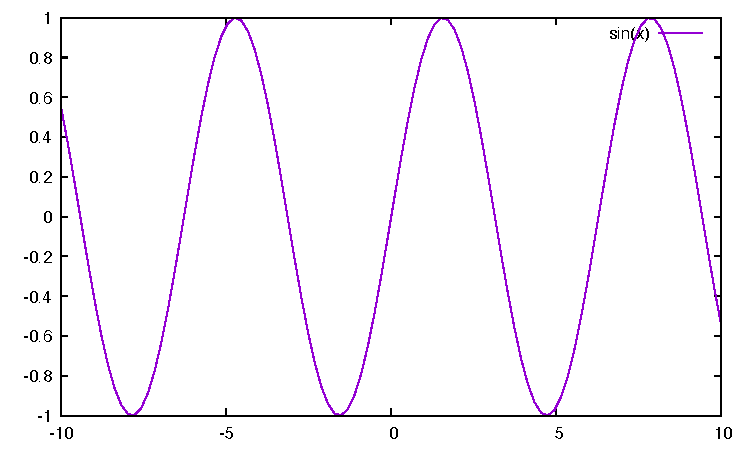
\includegraphics[width=0.9\linewidth]{demo.pdf}
        \captionof{figure}{}
        \label{fig:placeholder}
    \end{minipage}
 
\end{minipage}\\
Pamiętaj zatem, żeby na bieżąco zapisywać wprowadzone do terminala polecenia.

\begin{enumerate}
    \item Korzystając z konstrukcji \verb|with (x/y/xy)errorbars| nanieś na wykres punkty z pliku \textit{dane1.dat}, używając odpowiednich kolumn.

    \item Powtórz to samo polecenie, ale teraz nie używaj do wyrysowania błędów numerów kolumn, tylko wyrażeń (wyrażenia obejmujemy w nawiasy). Niech błąd z osi $x$ będzie stały i wynosi $1$, natomiast w osi $y$ niech będzie równy pierwiastkowi z wartości współrzędnej $y$ punktu (wskazówka: w wyrażeniach do kolumn odwołujemy się przez \verb|$1,$2,|\dots).
    \item Do danych z plików \textit{dane2a.dat} dopasuj krzywe sklejane przy pomocy \verb|acsplines|, jednocześnie nanosząc na wykres punkty z pliku. Pierwsze dwie kolumny to odpowiednio współrzędne $x$ oraz $y$, a trzecia kolumna to wagi, określające jak duży wpływ na dopasowanie krzywej mają poszczególne punkty. \\
    Nanieś na wykres również krzywą dopasowaną do pliku \textit{dane2b.dat}. Zwróć uwagę na zmienione wagi i wytłumacz to zachowanie.
    \item Zdefiniuj funkcję $f(x)$ jako funkcję liniową zależną od dwóch nieznanych parametrów $a$ i $b$
    \begin{verbatim}
        f(x)=a*x+b.
    \end{verbatim}
    Następnie, dopasuj ją przy pomocy polecenia $fit$ do danych z pliku \textit{dane1.dat}. Ostatecznie, przy pomocy \verb|plot f(x)|.
    Następnie uwzględnij przy dopasowaniu niepewności w zmiennej $y$ (\verb|yerr|). Zaobserwuj ich wpływ na dopasowaną funkcję.
    \end{enumerate}
\end{document}